\documentclass[a4paper]{jpconf}
\usepackage{graphicx}
\begin{document}
\title{Powering physics data transfers with FDT}

\author{Zdenek Maxa$^1$, Badar Ahmed$^2$, Dorian Kcira$^1$,
Iosif Legrand$^1$, Azher Mughal$^1$, Michael Thomas$^1$,
Ramiro Voicu$^1$}


\address{$^1$ California Institute of Technology, Pasadena, California, USA}
\address{$^2$ National University of Science and Technology, Pakistan}

\ead{zdenek.maxa@hep.caltech.edu}


\begin{abstract}
We present a data transfer system for the grid environment built on top of the
open source FDT tool (Fast Data Transfer) developed by Caltech in
collaboration with the National University of Science and Technology
(Pakistan). The enhancement layer above FDT consists of a client program -
fdtcp (FDT copy) and a fdtd service (FDT daemon). This pair of components
allows for GSI authenticated data transfers and offers to the user (or data
movement production service) interface analogous to grid middle-ware data
transfer services - SRM (i.e. srmcp) or GridFTP (i.e. globus-url-copy).
fdtcp/fdtd enables third-party, batched file transfers. An important aspect is
monitoring by means of the MonALISA active monitoring light-weight library
ApMon, providing real-time monitoring and arrival time estimates as well as
powerful troubleshooting mechanism.

The actual transfer is carried out by the FDT application, an efficient
application capable of reading and writing at disk speed over wide area
networks. FDT's excellent performance was demonstrated e.g. during
SuperComputing 2009 Bandwidth Challenge.

We also discuss the storage technology interface layer, specifically focusing
on the open source Hadoop distributed file system (HDFS), presenting the
recently developed FDT-HDFS sequential write adapter.

The integration with CMS PhEDEx is described as well.
The PhEDEx project (Physics Experiment Data Export) is responsible for
facilitating large-scale CMS data transfers across the grid.

Ongoing and future development involves interfacing with next generation
network services developed by OGF NSI-WG, GLIF and DICE groups, allowing for
network resource reservation and scheduling.
\end{abstract}


\section{Introduction} % ####################################################
The distributed computing model of the CMS~\cite{cms} experiment relies
heavily on effective
utilisation of network links. The aim is to transfer data in
as efficient and reliable fashion as possible. Such a need is similar to
any experiment generating huge amounts of data that are necessary to
distribute around the globe.

Although the main motivation for this presented study and project came
primarily from CMS, the {\bf fdtcp} grid transfer tool built on top of FDT
can be used used in any experiment or collaboration requiring third-party,
grid environment authenticated transfers.


\subsection{Motivation}
The transfer performance measurements discussed in the
section~\ref{benchmarks} done over WAN
links CERN - Caltech, USA and FDT's excellent performance record
on the SuperComputing conferences~\cite{fdtsc09} suggested that it's
worth to
extend FDT capabilities into the grid environment.
The experiments proved that the CMS data transfers, but also any data
transfers-intensive experiment in general, would benefit from increased
performance if FDT was used on the lowest lever of the transfer
stack (e.g. as an alternative to GridFTP).

Another future aspect is the intention to employ dynamic network circuits
provisioning~(\ref{dynes}). 


\subsection{FDT Characteristics} % ##########################################
Fast Data Transfer (FDT)~\cite{fdt}, also referred to as \emph{FDT Java},
is an application capable of reading and
writing at disk speed over wide area links. Written entirely in the Java
language, it uses merely TCP sockets, Java NIO (New
I/O) and direct memory buffers. It is based on the client-server model, is
heavily multi-threaded and supports batched
transfers\footnote{A set of files in the transfer from A to B is processed
by a single pair \{client, server\} as opposed to the grid middle-ware
GridFTP, which launches fresh instances of GridFTP \{client, server\} for
each file in the batch.}. 

Given the parallel nature of FDT, there is a major performance gain over WAN
links (high RTT - Round Trip Time). Similarly to GridFTP, the FDT uses
multiple TCP sessions. A novel concept is transferring
files in a job in parallel (another level of parallelism above
simultaneous TCP sessions), which provides a significant performance boost
between distributed storages (e.g. Hadoop~\cite{hdfs} or
Lustre~\cite{lustre}).

It is distributed as an open-source project and has been developed by
Caltech. The project is for example used by NOAA~\cite{noaa}.

The FDT transfer can be very easily and seamlessly connected to the MonALISA
monitoring framework that enables real time transfer monitoring - invaluable
capability for network problems investigation.

Although FDT has a number of security features (source IP filtering, SSH,
GSI\footnote{Grid Security Infrastructure.}-SSH, GSI-enabled server) it is not
capable of managing third-party, grid-authenticated (GSI)
transfers\footnote{FDT features third-party transfers but only via SSH
and such access is generally not given to users in the grid environment.}.


\section{Transfer performance benchmarking} % ###############################
\label{benchmarks}

There has been a number of transfer performance measurements and comparisons
conducted. The page~\cite{transfer} summarizes all initial experiments
(with plain FDT before the enhancing fdtcp layer was developed) as well as
analogous final comparisons between {\bf globus-url-copy} (GridFTP), {\bf
srmcp} (SRM) and {\bf fdtcp}. This section discusses and interprets the
final results\footnote{1 file in parallel means that parallel files files
is not used or the feature is not available.}.

\begin{center}
\begin{table}[h]
\centering
\caption{\label{benchtable} srmcp, globus-url-copy and fdtcp
performance comparison (100x1GB transfer job)}
\begin{tabular}{@{}l*{15}{l}{l}{l}{l}}
\br
application & parallel streams & parallel files & time [min] &
    performance [MB/s] \\
\mr
globus-url-copy & 35 & 1 (n/a) & 74 & 23 \\
srmcp & 35 & 1 (n/a) & 80-120 & 14-21 \\
fdtcp & 35 & 1 & 41 & 42 \\
fdtcp & 35 & 12 & 8-12 & 142-213 \\
\br
\end{tabular}
\end{table}
\end{center}


The benchmarking was carried out from the Caltech cluster at CERN to the
Caltech campus cluster in California having distributed storages
HDFS (Hadoop)~\cite{hdfs} at both ends. The following list
summarizes attributes of these tests:

\begin{itemize}
\item memory to memory transfer between the clusters was 7.2Gbps
(900MB/s) (link capacity),
\item a transfer job consists of 100 files of 1GB in size,
\item measured values of time come from the GNU/Linux \emph{time} utility,
so all
overhead of the application, resp. protocol is taken into account (e.g. time
spent in authentication, etc),
\item unless specified, the SRM, resp. GridFTP tests were done using
default values (e.g. buffer sizes, etc).
\end{itemize}

srmcp doesn't perform any data transfers physically itself, it calls
GridFTP, resp. globus-url-copy to conduct the
actual data movement. The comparison of results srmcp vs. globus-url-copy then
just shows the srmcp's overhead on top of GridFTP. This is why only
fdtcp vs globus-url-copy comparison is relevant\footnote{The FTS, another
transfer service used e.g. by CMS PhEDEx system, delegates the transfer either
to SRM (which cascades to GridFTP) or directly to GridFTP.}. In order to
interpret the superior fdtcp, resp. FDT performance over GridFTP, it's
necessary to realise following aspects:

\begin{itemize}
\item The feature of transferring files in parallel (fdtcp) specifies 12
parallel files. This value is configurable in the fdtcp application and shall
reflect the size of the storage cluster. If this was used in case of 1
storage node, it would lead to unnecessary transfer context switching and
congestion, it is only useful in case of distributed storages,

\item GridFTP doesn't have the above feature. As the
table~\ref{benchtable} shows, this is where fdtcp gains major boost over
GridFTP.
Taking into account the fact that an experiment's, like CMS, huge
amounts of data are always\footnote{Not considering tape storage.}
accommodated in a distributed storage\footnote{dCache, Hadoop, Lustre.}, it is
a major drawback that the only currently used transfer
technology doesn't provide such functionality, which lack of appears to be a
chief contributor to the network links being utilized suboptimally, 

\item Another observed characteristic of GridFTP transfers
was that for each file in
the sequence (batch) is launched a new pair of source-destination transfer
applications - obvious overhead shutting and restarting the application.
Also, the authentication is performed for each file in the
batch. In the light of these facts, FDT can already be considered roughly
twice as fast compared to GridFTP, even when parallel files are not 
enabled in FDT.
This is only true with respect to the fileset features (100x1GB), as the
following table~\ref{benchtable2} demonstrates\footnote{FDT was used directly
in this case, without the extension fdtcp layer.}.
\end{itemize}


\begin{center}
\begin{table}[h]
\centering
\caption{\label{benchtable2} FDT, GridFTP transferring a single
large file (1x100GB), no parallel files.}
\begin{tabular}{@{}l*{15}{l}{l}{l}}
\br
application & parallel streams & time [min] & performance [MB/s] \\
\mr
globus-url-copy & 35 & 29.5 & 57.9 \\
FDT & 35 & 28.9 & 59.1 \\
\br
\end{tabular}
\end{table}
\end{center}

The table~\ref{benchtable2} shows equal performance of FDT vs. GridFTP
in case of 1x100GB transfer job, i.e. only one large file. Compared to
the results in the table~\ref{benchtable}, this presents performance
increase of 40\% in
case of FDT and 152\% in case of GridFTP. The latter is significantly
retarded by the circumstances discussed above in case of many files in the
transfer job, e.g. 100x1GB. The reached rate values in the
table~\ref{benchtable2} are limited by the storage / filesystem
performance regardless of the transfer protocol.

We conclude that, above
reliable functionality, the optimal utilisation of the network links, which
to a large degree translates into transfer protocol performance, is an
important aspect. The argument that the traditional
grid middle-ware service (GridFTP) can transfer files equally effectively
when launched independently in parallel multiple instances is at least
disputable: launching
parallel transfer application instances in situations where performance of
those applications shall be examined and questioned consumes unnecessary
amounts of resources.
Additional resources must be provided by additional physical nodes
whose support and maintenance consumes extra both human and financial
resources. In this context, we would like to quote~\cite{haipheng}: "More
GridFTP\footnote{More GridFTP servers - reader, writer pairs.} increases the
total throughput of the system\footnote{Cluster of storage nodes.} and
reduces individual server's throughput.". This is an important system
administration observation suggesting investigations into optimal
utilisation of resources.


\section{Architecture \& Implementation of fdtcp} % #########################
The scheme~\ref{fdtcppic} displays the main blocks and the data,
resp. control flow among them.

\begin{figure}[h]
\begin{minipage}{9cm}
\includegraphics[height=4cm]{../img/fdtcp.eps}
\caption{\label{fdtcppic}fdtcp transfer application design.}
\end{minipage}\hspace{1cm}
\begin{minipage}{3.7cm}
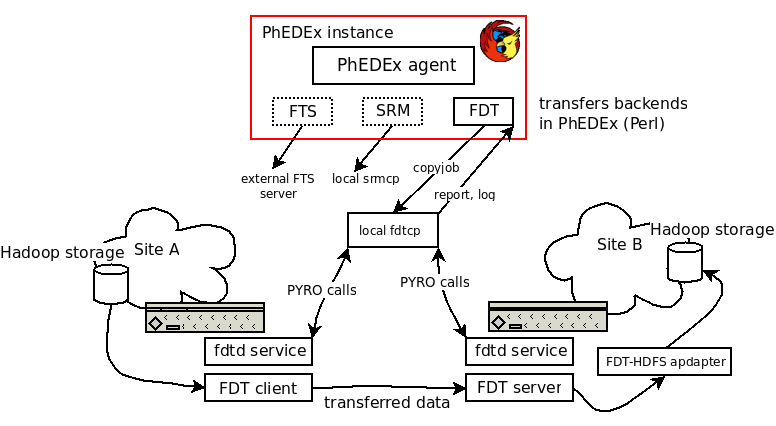
\includegraphics[height=4cm]{../img/phedex-fdt.eps}
\caption{\label{phedexfdtpic} PhEDEx integration}
\end{minipage} 
\end{figure}


\begin{itemize}
\item {\bf fdtcp} is a Python client component that can be used
analogously to srmcp\footnote{The fdtcp/fdtd pair doesn't provide any
services beyond data movements, no remote files management like SRM does.},
it can be fed the batch specification - \emph{copyjobfile} and
generates \emph{reportfile} as required by PhEDEx,
\item {\bf fdtd} is a Python daemon, counterpart to fdtcp, utilizing 
PYRO~\cite{pyro} technology (RPC\footnote{Remote Procedure Call.}), runs at
sites, fdtd performs following requests from fdtcp:
\begin{itemize}
\item grid authentication and mapping to local grid users against gridmap file
\item launching FDT Java reader, resp. writer processes under local accounts
\end{itemize}
\item {\bf FDT Java} (represented by a single \emph{fdt.jar} file) - Java
processes started / stopped on demand from fdtd, the writer (usually the
destination party) will only respond to certain IP address (reader party),
this service
needs to run at sites supporting \emph{fdt} protocol (analogously to GridFTP),
\item {\bf FDT-HDFS} - Hadoop storage (HDFS) is capable of writing only
sequential data (which contradicts the parallel nature of FDT transfers). This
adapter layer serializes arriving data into a form, which can be written into
HDFS
space in sequential fashion. This adapter component has also been developed
within this project and it should be noted that for instance with Lustre
store~\cite{lustre} it would not be necessary. 
\end{itemize}


\subsection{FDT-PhEDEx integration}
This section enters the realm of CMS, which specifically means interfacing
fdtcp and the PhEDEx system\footnote{PhEDEx is the CMS production system
responsible for data movements, utilises FTS
(File Transfer Service) or SRM and by means of this project also FDT. 
Further information on the PhEDEx system can be found in the
resources~\cite{phedex,phedexweb}.}.

As shown in the~\ref{phedexfdtpic} schema,
the frontier is defined by FDT ({\bf FDT.pm}) component within the PhEDEx
instance. The download agent is a daemon, which periodically polls the
central PhEDEx database for scheduled work on a given network link
(e.g. Nebraska - Caltech). The FDT.pm module invokes fdtcp,
feeding it with prepared copyjobfile (list of \emph{source, destination}
pairs\footnote{fdt://t3-fdt.ultralight.org:8444/mnt/hadoop/path/to/file1
fdt://gridftp01.ultralight.org:8444/mnt/hadoop/path/to/file2}), receives
back reportfile with transfer results.
The currently supported transfer backends by PhEDEx are: SRM, FTS,
FDT as shown in the picture~\ref{phedexfdtpic}.

In general it should be noted that FDT transfers by means of fdtcp can be used
in situations where SRM, resp. srmcp is currently used (fdtcp and srmcp have
analogous command line interface) and there is a need for better and optimal
network utilisation. Up to the fdtcp level, the presented
transfer technology is entirely independent on the CMS experiment systems.


\subsection{Grid Authentication}
The authentication mechanism currently used by fdtcp, fdtd when interacting
with the host system is based on \emph{gridmapfile}. This vehicle is used in
both European as well as American grid environments, though in the latter is
often complemented by a preferred GUMS system~\cite{gums}. It is one of the
future work items to implement GUMS support across fdtcp, fdtd.

\subsection{FDT Transfer Monitoring}

\begin{figure}[h]
\includegraphics[height=4.5cm,width=11cm]{../img/100GBtransfer-01-final.eps}
\hspace{0.5cm}
\begin{minipage}[b]{4cm}
\caption{\label{mlpic1} Hadoop - Hadoop 100x1GB files transfer CERN - 
Caltech T2 (California) reaching 107~MB/s via 1Gbps interface}
\end{minipage}
\end{figure}


FDT Java as well as fdtcp, fdtd and fdt-hdfs components
are (very loosely) coupled with the MonALISA monitoring
framework~\cite{monalisa}. Each transfer executed by fdtcp is equipped with a
unique transfer id, which can be used to track, trouble-shoot and monitor.
Inspecting the progress of the transfer can currently be done via a
web-executable MonALISA client application (groups \emph{FDT\_MON}), however
a web browser-accessible repository can easily be enabled.

The plot~\ref{mlpic1} shows almost saturated 1Gbps network
interface. The long
string on top of the picture is the transfer id. The peaks exceeding 1Gbps
threshold are caused by buffering effect.


\section{Current Status and Future Work} % ###################################
The FDT transfers have been thoroughly tested in the grid environment. The
installation of the component stack has been done on CMS T2 sites Caltech and
Nebraska and PhEDEx instances at these sites were configured to utilise FDT
for so
called \emph{debug transfers} (as opposed to production transfers).
Once enough experience and
confidence is gathered, the FDT protocol will be used for production
transfers among selected sites. The
page~\cite{phedexfdt} lists details on progress of FDT-PhEDEx integration as
well as instructions for PhEDEx administrators on how to evaluate this
alternative transfer application.

However, the project is still under development. The main planned work
items involve:
\begin{itemize}
\item Further ease of installation and configuration (largely
automated from RPM packages),
\item Gather more experience / performance observation and eventually
comparison of FTS vs FDT transfers from within PhEDEx (PhEDEx transfer rate,
plots) - performance study in the production CMS environment,
\item Similarly to Hadoop-Hadoop performance tests, Lustre tests are planned,
\item Evaluation of using GUMS for local grid user mapping (complement to the
current gridmap file) and using \emph{glExec},
\item Capability of utilisation of provisioned dynamic circuits
(DYNES).
\end{itemize}

\subsection{DYNES - Dynamic Network System}
\label{dynes}
The DYNES~\cite{dynesref} is a project funded by USA NSF and is aimed at
creating a dynamic network "cyber-instrument" spanning ~40 US universities
and ~14 Internet2 connectors featuring scheduling, planning and provisioning
dynamic network circuits for large transfers of scientific data.

The integration of FDT and dynamic network circuits capability was
successfully demonstrated at GLIF 2009 meeting (Global Lambda Integrated
Facility). This integration scenario happens on the FDT Java level and is
therefore entirely transparent to PhEDEx as far as CMS is concerned.


% ###########################################################################


\ack
This work was supported by the National Science Foundation within the DISUN
grant, contract No. PHY-0533280, by the National Science Foundation within the
Ultralight grant, contract No. PHY-0427110.


\section*{References}
\begin{thebibliography}{2}
\bibitem{cms} CMS - Compact Muon Solenoid CERN experiment
{\it http://cms.cern.ch}
\bibitem{fdt} Fast Data Transfer (FDT) {\it http://monalisa.cern.ch/FDT}
\bibitem{fdtsc09} FDT SuperComputing 2009 conference bandwidth challenge
{\it http://monalisa.cern.ch/FDT/sc09.html}
\bibitem{phedexfdt} FDT and PhEDEx integration summary {\it
https://twiki.cern.ch/twiki/bin/view/Main/PhEDExFDTIntegration}
\bibitem{phedexweb} CMS PhEDEx website 
{\it https://twiki.cern.ch/twiki/bin/view/CMS/PhEDEx}
\bibitem{phedex} Ricky Egeland, Tony Wildish, Simon Metson 2008 Data
transfer infrastructure for CMS data taking {\it XII Advanced Computing and
Analysis Techniques in Physics Research, November 3-7 2008 Erice, Italy}
\bibitem{transfer} Transfer performance benchmarking summary 
{\it https://twiki.cern.ch/twiki/bin/view/Main/TransferPerformance}
\bibitem{srm} SRM - Storage Resource Management 
{\it https://sdm.lbl.gov/srm-wg}
\bibitem{hdfs} HDFS - Apache Hadoop Distributed File System 
{\it http://hadoop.apache.org/hdfs}
\bibitem{lustre} Lustre - Oracle Distributed File System
{\it http://wiki.lustre.org}
\bibitem{noaa} NOAA - National Oceanic and Atmospheric Administration
{\it http://www.noaa.gov}
\bibitem{monalisa} MonALISA - MONitoring Agents using a Large Integrated
Services Architecture {\it http://monalisa.cern.ch}
\bibitem{dynesref} DYNES - Dynamic Network System 
{\it  http://www.internet2.edu/dynes}
\bibitem{haipheng} Haifeng Pi 2010 High Throughput WAN Data Transfer
with Hadoop-based Storage (PS23-4-071)
{\it CHEP 2010, October 18-22, 2010 Taipei, Taiwan}
\bibitem{pyro} PYRO - Python Remote Objects
{\it http://www.xs4all.nl/~irmen/pyro3}
\bibitem{gums} GUMS Grid User Management System
{\it https://www.racf.bnl.gov/Facility/GUMS/1.3}
\end{thebibliography}
\end{document}

% grid low case
% may list some details of how real CMS transfers are done - info on Phedex
%   from Tony, Mike

